\documentclass[modern]{aastex61}
\usepackage{hyperref}
\usepackage{xspace}
\usepackage{booktabs}
\usepackage[utf8]{inputenc}
\usepackage[T1]{fontenc}
\newcommand{\escapecmd}[1]{\texttt{\detokenize{#1}}}

\submitjournal{ApJ}

\shorttitle{Astropy Project II}
\shortauthors{Astropy Project et al.}

% Packages / projects / programming - for consistency!
\newcommand{\package}[1]{\texttt{#1}\xspace}
\newcommand{\github}{\package{GitHub}\xspace}
\newcommand{\python}{\package{Python}\xspace}
\newcommand{\astropy}{Astropy\xspace}
\newcommand{\astropypkg}{\package{astropy}\xspace}

% For consistency:
\newcommand{\sectionname}{Section\xspace}
\renewcommand{\figurename}{Figure\xspace}
\newcommand{\equationname}{Equation\xspace}
\renewcommand{\tablename}{Table\xspace}

% For commenting - can be deleted before submission
\usepackage[colorinlistoftodos]{todonotes}
\newcommand{\inlinecomment}[2]{\todo[inline]{#1: #2}\xspace}
\newcommand{\comment}[2]{\todo{#1: #2}\xspace}

\begin{document}

\draft{\today}

\title{The Astropy Project}

\correspondingauthor{Astropy Coordination Committee}
\email{coordinators@astropy.org}

\author{Astropy Collaboration}

\begin{abstract}
% I (Adrian) took a first stab at the abstract, but it needs some work. Feel
% free to modify!
The \astropy project supports and fosters the development of open-source and open-development
\python packages that provide commonly-needed functionality to the astronomical
community.
A key element of the project is the \astropy core package, which serves as the
foundation for more specialized projects and packages.
In this article, we provide an overview of the organization of the \astropy
project and summarize key features in the core package as of the recent major
release, version 2.0.
We then describe the project infrastructure designed to facilitate and support
development for a broader ecosystem of inter-operable packages.
We conclude with a future outlook of planned new features and directions for the
broader \astropy project.
\end{abstract}

%% Keywords should appear after the \end{abstract} command.
%% See the online documentation for the full list of available subject
%% keywords and the rules for their use.
\keywords{}

\section*{\textit{Notes and guidelines (to be removed)}}

\begin{itemize}
   \item The goal is to produce a brief and informative paper that covers major
        \astropy principles not mentioned in the first paper, the core v2.0
        package, and infrastructure in \astropy project to support development
        in \python.
    \item We don't plan on including code in this paper, but if you think you
        will need to include code in your section, please add it to a separate
        Python module (.py file) and include it in this repository.
    \item Use \escapecmd{\sectionname} not ``Section,'' \escapecmd{\figurename}
        not ``Figure''
    \item Use \escapecmd{\astropypkg} for the astropy package,
        \escapecmd{\astropy} for the astropy project, \escapecmd{\python} not
        ``Python''
    \item If your subpackage was included in Paper I, then please just include a
        note on what the package does, a reference to paper I, and any new major
        updates to your package
    \item If your subpackage was not included, then please describe the
        sub-package on level with what was in the first paper, and highlight any
        major features in it. Typical length should be equivalent to one page
        (single-column).
    \item Please make sure you are logged into Overleaf or pushing a commit with
        your information to be able to track the contributors to the paper.

\end{itemize}

\section{Introduction} \label{sec:intro}
% first draft by Moritz (hamogu)
All astronomical research makes use of software in some way and
astronomy as a field has long supported the development of specialized
software tools for different astronomical tasks. Some of those
software packages are (or at least were) supported by large
institutions, e.g.\ IRAF \citep[developed at NOAO,][]{IRAF}, MIDAS
\citep[developed at ESO,][]{MIDAS}, or ds9 \citep[developed at
% * <bsipocz@gmail.com> 2017-09-28T21:05:00.569Z:
%
% > or ds9
% probably starlink is a better example as being a large package of software similarly to IRAF and MIDAS rather than a single tool.
%
% ^.
% hamogu: Feel free ot swap in Starlink, if you think that's more appropriate. I picked ds9 becase (a) it's wider known (e.g. in the X-ray community) and (b) because it is an example of a widely used tool with institutional support that is NOT a large package. TOPCAT would have been another example if we want to expand that list.
% olebole: TOPCAT is part of Starlink Java. An other examples would be CASA resp. AIPS. I'd rather omit ds9, since it is mainly developed by one person. 
  SAO,][]{ds9}. These packages tend to address a wide range of users
and typically provide some level of documentation and user
support is provided. Other packages are developed foremost by individual research
groups and used mostly in work by members of the group. Those
packages can address more specialized needs, but are not necessarily
available to the community and even if they are, documentation can in
some cases be insufficient for new users and the quality of the
software, i.e.\ the robustness and the level of testing that has been
performed to ensure correctness, is not always clear. On the other
hand, there are also many widely used, well documented, high quality
software packages which are developed by individuals or small groups.

The implementation of astronomical software, be it for a package meant
for wide distribution or scripts and programs for a specific research
project, can be eased by the use of a library that provides core
functionality that is common to many astronomical tasks. Reading and
writing FITS files is one example where it is time
consuming to implement the FITS standard correctly and
programming is much faster when using an existing library to perform this
task. Another example of such a common task is dealing with different
astronomical coordinate systems. The \astropy project aims to provide a
library of core astronomical functionality in the \python programming
language.

\python\footnote{\url{https://www.python.org/}} is an increasingly popular
general-purpose scripting language that is available under a permissive open
source software licence free of charge for all major operating systems. Stable
and well-developed packages provide support for array arithmetic
\citep[\package{numpy},][]{numpy}, a wide variety of functions for scientific
computing \citep[\package{scipy},][]{numpy}, and publication-quality plotting
\citep[\package{matplotlib},][]{matplotlib}. Tens of thousands of other packages
are available which can help with tasks that are not astronomy specific but
might be performed in the course of astronomical research, e.g.\ presenting
results on websites or interfacing with databases.

At the same time, an ecosystem of tools, programs, and webservices
has become available that makes it easier to collaborate on code development,
continuously test the code, build and provide documentation, and
supply downloadable packages. The \astropy project aims to develop and
provide high quality code and documentation according to the best
practices in software development. The project makes use of these
tools to do so without central institutional oversight.

The first public release of the \astropy package is described in
\cite{astropy}. Since then, the \astropy package has been
used in hundreds of projects, and the scope of the package has grown
considerably. At the same time, the community of astronomers
contributing to the project has grown tremendously and an ecosystem
of packages supporting or affiliated with the \astropy core has
developed. In this paper, we describe the current status of the
\astropy community, the \astropy core package, and the \astropy\
ecosystem.

We start by describing the way the \astropy project works and is
organized in \sectionname~\ref{sec:concepts}.  The project develops a core
package called \astropypkg (\sectionname~\ref{sec:core}) and several
separate packages that help setting up the infrastructure for testing,
documentation etc.\ (\sectionname~\ref{sec:infrastructure}). 
We end with a short vision for
the future of \astropy in particular and astronomical software in general
in \sectionname~\ref{sec:future}.


\section{Major concepts}
\label{sec:concepts}
% Anyone want to take this??

\subsection{Coordination of Astropy}
\inlinecomment{Kelle}

\subsection{APEs - Astropy Proposals for Enhancement}
%draft by hamogu
Central to the success of \astropy is an open environment where
anybody can contribute to the code by opening a so-called ``pull
request'' with a new code contribution on a publically available
website\footnote{\url{https://github.com/astropy/astropy}}; this
request is then reviewed by at least one of the maintainers responsible for the specific
sub-package and possibly merged into the main code base. Most bug
fixes and small features are contributed in this way. However, this
model leads to ``organic'' growth where different features are
implemented by different people with different programming styles and
interfaces. Thus, \astropy has a mechanism to more formally propose
changes to the code management (e.g.~the release cycle) or to plan
out major new features. This mechanism is called ``Astropy Proposal
for Enhancement'' (APE). In an APE one or more authors lay out a
vision for a new feature, including a rationale why this feature is
needed, how it should be implemented, and what the interface will
be. These APEs are discussed and refined before much work is invested
into a detailed implementation. APEs are again edited and discussed on
a platform\footnote{\url{https://github.com/astropy/astropy-APEs}}
open to the public. In previous APEs a community consensus emerged and
APEs are accepted and become the basis for future work at this
point. In cases where consensus cannot be reached, the
\astropy coordination committee can decide to close the discussion and
make an executive decision based on the community input on the APE in
question. APEs are modeled after the ``Python Enhancement Proposals''
(PEP) and guide the development of the \python programming language.


\subsection{Astropy development model, astropy ecosystem}
\inlinecomment{Needs writing by EJT}

This subsection should include some basic statistics about the contributors, commits, line of code etc. up to the 2.0 release when we know it.

\subsection{Concept of affiliated packages}
% it may be described in previous subsection, if not the Brigitta can try to
% write it up
%
\par A major part of the \astropy~project is the concept of
``Affiliated Packages''. An affiliated package is an astronomy-related
\python~package that is not part of the \astropypkg~core package, but
has requested to be included as part of the \astropy project's
community. These packages support the goals and vision of \astropy~of
improving code reuse, interoperability, and embracing good coding
practices such as testing and thorough documentation. \astropypkg{}
version 2.0 supports \python~2.7 and \python~3.4+, affiliated packages
are strongly encouraged to support at least \python~3.x.
%
\par Affiliated packages contain functionality that is more specialized, or
have license incompatibility, or have enough external dependencies (e.g. GUI
libraries) that limit their integration possibility into the core and thus
they are more suitable to be separate packages. Starting as an affiliate 
package is also seen as a good strategy for functionality that is aimed for
the \astropypkg~core but is initially undergoing rapid development and can 
benefit from a different release cycle while stabilizing its API. 
%
\par In general we hope that becoming an affiliated package is seen as 
a good way for new and existing packages to gain exposure.
%
\inlinecomment{BMS}{TODO: write about the process of becoming affiliated, and project packages into the future section below}
%
%\subsection{Mixin}

%\subsection{Accuracy testing across many different implementation}

\subsection{Use of Quantities across package}
% Marten and Tom R.

{\bf Very rough first text!}

Historically, it has been unusual to keep units as part of numbers, especially as speed was often deemed essential and quantities used to be slower than regular arrays. Hence, programs and functions expected to be fed parameters in particular units, as (hopefully) stated in their documentation.  In \astropypkg~0.4, therefore, unit and quantity support was still somewhat spotty, but this has changed greatly.  One of the riskiest classes was angles, where both degrees and radians were ``obvious'' default units to some. As a consequence, quantities are most fully integrated in the coordinates module (\sectionname~\ref{sec:coordinates}). In \astropypkg~2.0, one can also opt in to use quantities fully in tables, by using the {\tt QTable} class (see \sectionname~\ref{sec:table}). As a result, units in FITS tables are also well-supported. For most other modules, quantities are at least accepted, and often assumed by default.

In the process, some standard wrappers have been defined that make defining functions that require quantities as input simpler. As an extension of this, we plan to define wrappers for functions that work on numbers that will automatically convert quantities to any required units.

\subsection{Release cycle and Long Term Support}
% This could also include information about the development cycle
% Brigitta can writes this up if there's no other taker
\inlinecomment{BMS: TODO}{reference APE2 for versioning and APE10 for dropping python2 support}
\inlinecomment{BMS}{shall we maybe refer to the release calendar, too?}
\inlinecomment{hamogu}{I don't think that's necessary. These details are in the docs, but not too important for a general paper.}
\inlinecomment{BMS}{should we mention that v3.0 is the exception to the
  version numbering scheme we use by not being 2.1?}
\inlinecomment{hamogu}{No. This is a genral paper, those are details that will be unimportant very soon. }
%
\par The general scheme for the releases and version numbering that the core
package has adopted if the following. \astropypkg has new feature releases every
6 months, and between feature releases additional bugfix releases that
contain only bugfixes but no new features.
% The timing of
%
\par Long-term support (LTS) releases continue to receive bugfixes for 2
years with no changes to the API\@. They are ideal for pipelines and other
applications where API stability is essential. The latest LTS release is
also the last one that supports \python 2, and will receive bug fixes until the
end of 2019.
%
\par The version numbering of \astropypkg reflects on the release scheme
described above. The core package uses the form x.y.z, where x is advances
on LTS, y is advanced for a non-LTS feature release, and z is advanced on
bugfix releases.

\subsection{Support of Astropy}

% This section should be a straight forward/factual description of the current
% funding and support provided to astropy with the purpose of explaining the
% current structure to the community

%\subsection{Difficulty of reversing design choices}
%Deciding if a feature should be included
%difficulty to decide where general use ends and "handy feature for some" starts, i.e. how to reject PRs or deal with maintenance burden

\section{Astropy Core Package v2.0}
\label{sec:core}

The \astropy project aims to provide \python-based packages for all tasks that
are commonly needed in a large subset of the astronomical community.
At the foundation is the \astropypkg core package, which provides general
functionality (e.g., coordinate transformations, reading and writing astronomical
files) or base classes for other
packages to utilize for a common interface (e.g., \texttt{NDData}).
In this section, we highlight new features introduced or substantially improved
since version v0.2 (previously described in \citealt{astropy}).

\inlinecomment{BMS}{The itemizations below look very weird being boldface under a much less prominent subsection title. would it be nicer in the final version if we leave it as is in the draft?}

% \subsection{Analytic Functions}
% moved to models and depreciated --
% just here for completeness at the moment
\inlinecomment{BMS}{I suggest to order the subsection lexicographically as reading the draft the current order seemed very random (unlike at the docs page where they the grouping logic is obvious)}
\subsection{Units and quantities}
\label{sec:units}
\inlinecomment{Marten, Adrian}{}

The \package{astropy.units} subpackage provides ...

\subsubsection{Key new features}

\begin{description}
    \item[Speed improvements] ...
    \item[Logarithmic units and magnitudes] ...
    \item[Interaction with \package{numpy} arrays] ...
\end{description}

\subsection{Constants}

\inlinecomment{David S.}

versioning


\subsection{Coordinates}
\label{sec:coordinates}
% Adrian, Erik

\subsubsection{Overview}
The \package{astropy.coordinates} subpackage is designed to support representing
and transforming celestial coordinates and, new in version 2.0, velocities.
The framework heavily relies on the \package{astropy.units} subpackage, and most
inputs to objects in this subpackage are expected to be \texttt{Quantity}
objects.
Some of the machinery also relies on the Essential Routines of Fundamental
Astronomy (ERFA) \texttt{C} library for some of the critical underlying
transformation machinery \citep{erfa}, which is based on the Standards Of 
Fundamental Astronomy (SOFA) effort \citep{sofa}.


A key concept behind the design of this subpackage is that coordinate
\textit{representations} and \textit{reference systems / frames} are independent
of one another.
For example, a set of coordinates in the International Celestial Reference
System (ICRS) reference frame could be represented as spherical (right
ascension, declination, and distance from solar system barycenter) or Cartesian
coordinates ($x$, $y$, $z$ with the origin at ).
They can therefore change representations independent of being transformed to
other reference frames (e.g., the Galactic coordinate frame).

The classes that handle coordinate representations (the \texttt{Representation}
classes) act like three-dimensional vectors and thus support vector arithmetic.
The classes that represent reference systems and frames (the \texttt{Frame}
classes) internally use \texttt{Representation} objects to store the coordinate
data---that is, the \texttt{Frame} classes accept coordinate data, either as a
specified \texttt{Representation} object, or using short-hand keyword arguments
to specify the components of the coordinates.
These preferred representation and short-hand component names differ between
various astronomical reference systems.
For example, in the ICRS frame, longitude and latitude are right ascension
(\texttt{ra}) and declination (\texttt{dec}), whereas in the Galactic frame, the
spherical angles are Galactic longitude (\texttt{l}) and latitude (\texttt{b}).
Each of the \texttt{Frame} classes define their own component names and
preferred \texttt{Representation} class.
The frame-specific component names map to corresponding components on the
underlying \texttt{Representation} object that internally stores the coordinate
data.
For most frames the preferred representation is spherical, although this is
determined primarily by the common use in the astronomical community.

Many of the \texttt{Frame} classes also have attributes specific to the
corresponding reference system that allow the user to specify the frame.
For example, the Fifth Fundamental Catalogue (FK5) reference system requires
specifying an equinox to determine the reference frame.
If required, these additional frame attributes must be specified along with the
coordinate data when a \texttt{Frame} object is created.
\figurename~\ref{fig:frame-transform-graph} shows the network of possible
reference frame transformations as currently implemented in
\texttt{astropy.coordinates}.
Custom, user-implemented \texttt{Frame} classes that define transformations to
any reference frame in this graph can then be transformed to any of the other
connected frames.

\begin{figure}
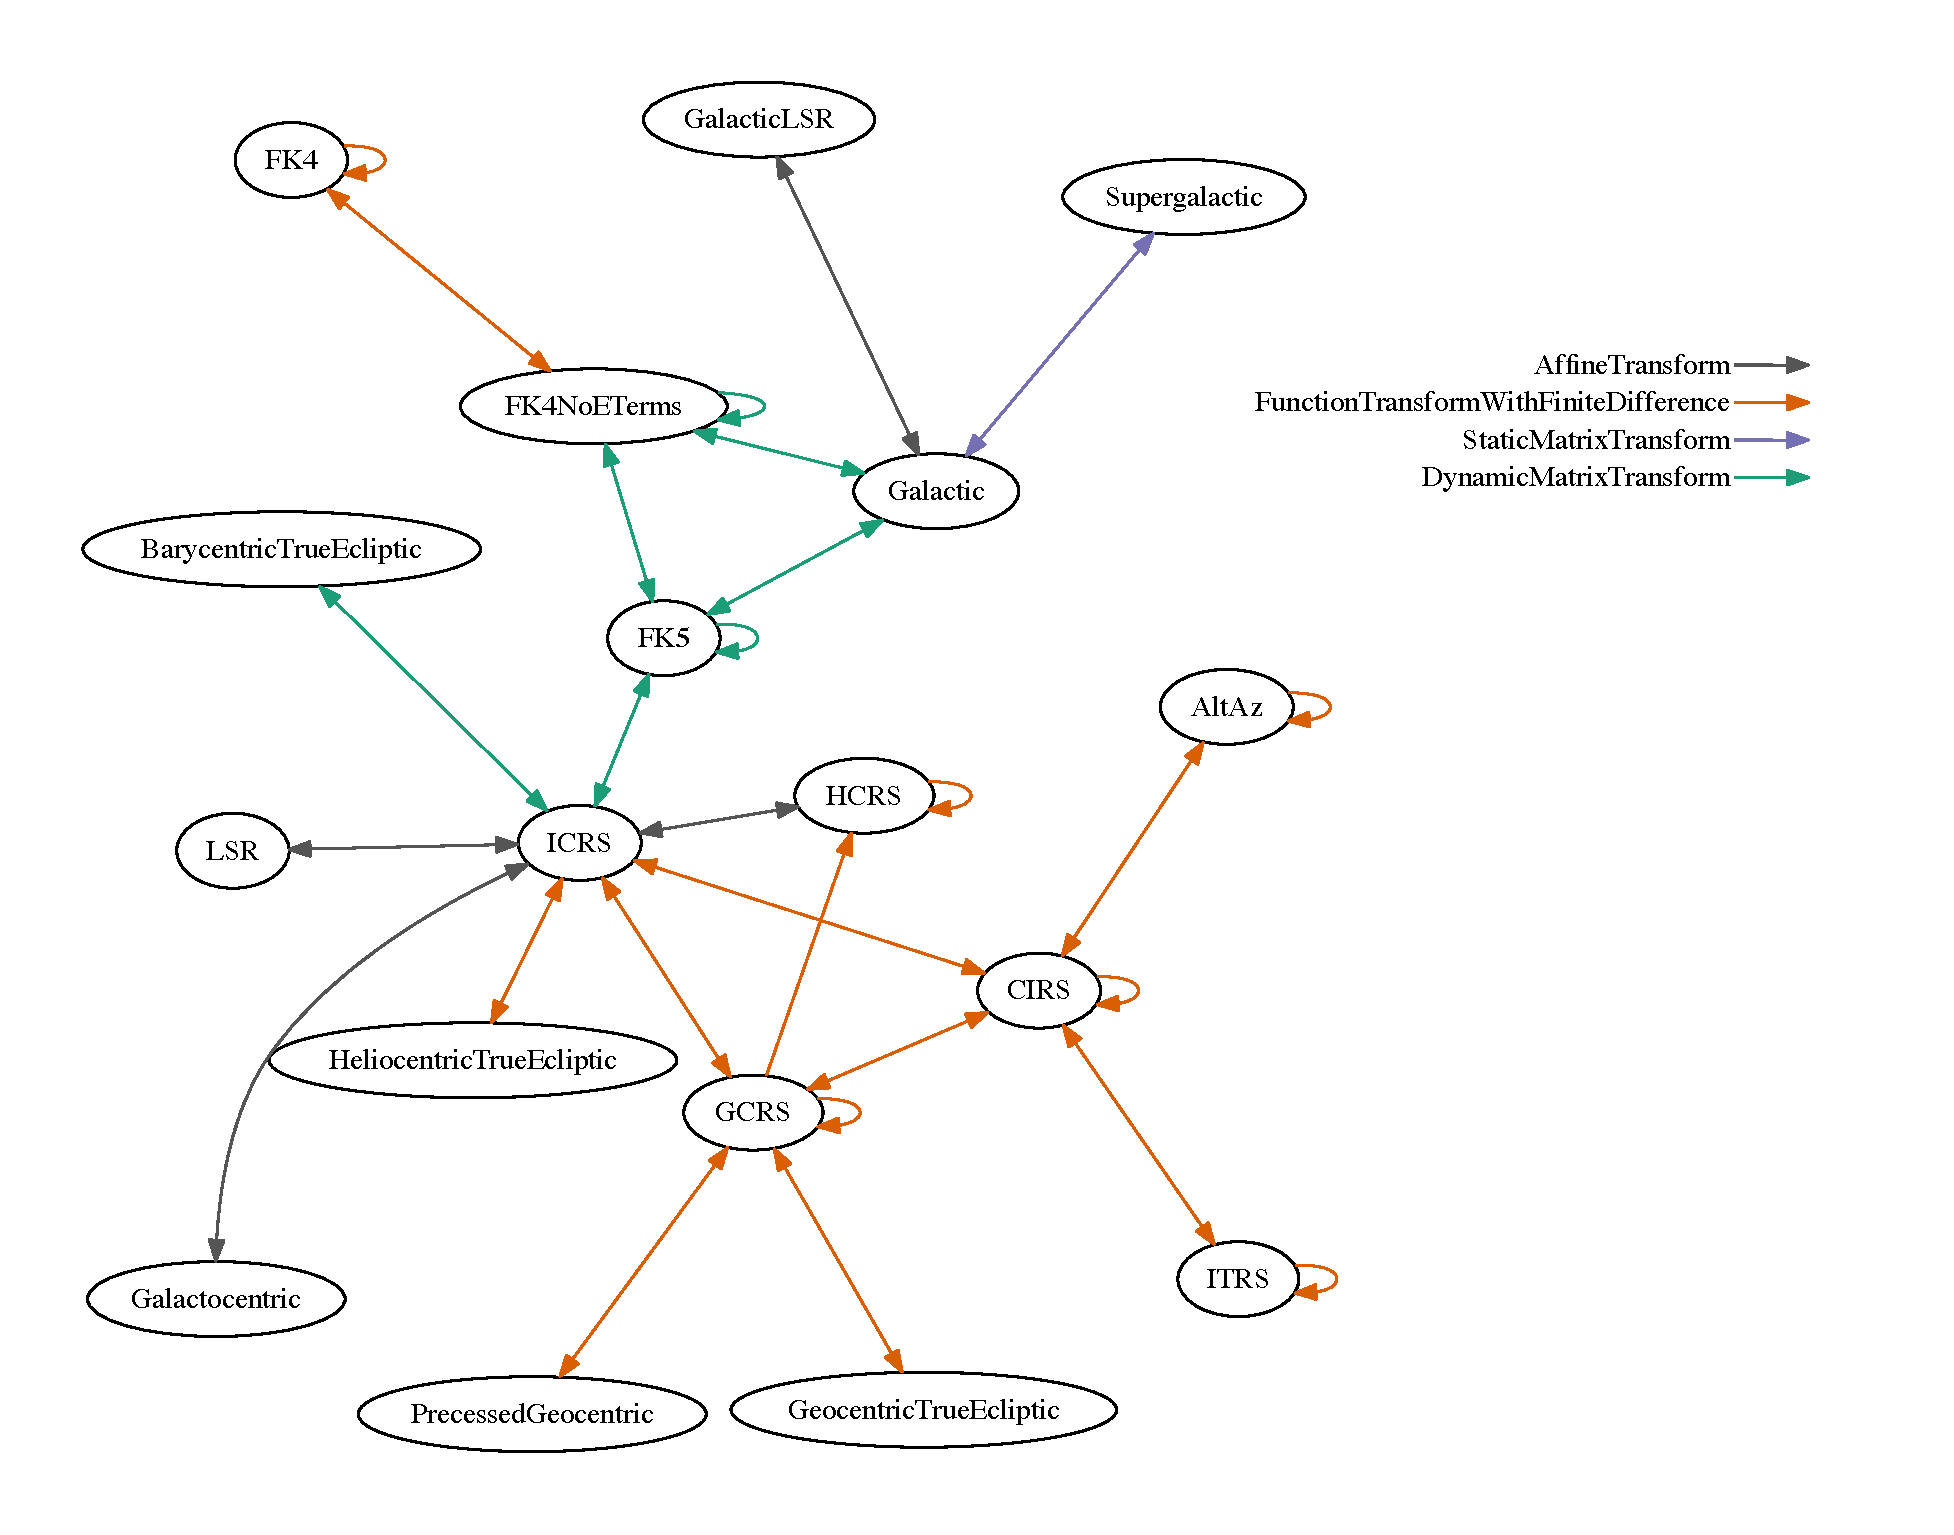
\includegraphics[width=\textwidth]{coordinates_graph.pdf}
\caption{%
    The full graph of possible reference frame transformations implemented in
    \texttt{astropy.coordinates}.
    \label{fig:frame-transform-graph}
}
\end{figure}

The typical user doesn't usually have to interact with the \texttt{Frame} or
\texttt{Representation} classes directly.
Instead, \texttt{astropy.coordinates} provides a high-level interface to
representing astronomical coordinates through the \texttt{SkyCoord} class.
The \texttt{SkyCoord} class was designed to provide a single class that
accepts a wide range of possible inputs.
It supports coordinate data in any coordinate frame in any representation by
internally using the \texttt{Frame} and \texttt{Representation} classes.

\subsubsection{Key new features}

\begin{description}
    \item[Local Earth coordinate frames] In addition to representing celestial
    coordinates, \astropypkg now supports specifying positions on the Earth in
    a number of different geocentric systems with the \texttt{EarthLocation}
    class.
    With this, \astropypkg now supports Earth-location-specific coordinate
    systems such as the altitude-azimuth (\texttt{AltAz}) or horizontal system.
    Transformations between \texttt{AltAz} and any Barycentric coordinate frame
    also requires specifying a time using the \texttt{Time} class from
    \texttt{astropy.time}.
    With this new functionality, many of the common tasks associated with
    observation planning can now be completed with \astropypkg or the
    \astropy-affiliated package \package{astroplan}\citep{astroplan_AAS}. 
    \inlinecomment{APW}{TODO: cite zenodo entry for astroplan?}
    \inlinecomment{BMS}{better to cite the submitted or soon to be submitted paper, I made a placeholder for it.}

    \item[Proper motion and velocity transformations]
    In addition to positional coordinate data, the \texttt{Frame} classes now
    also support velocity data.
    As the default representation for most frames is spherical, most of the
    \texttt{Frame} classes expect proper motion and radial velocity components
    to specify the velocity information.
    The names of the proper motion components all start with \texttt{pm} and
    adopt the same longitude and latitude names as the positional components.
    Transforming coordinates with velocity data is also supported, but in some
    cases the transformed velocity components have limited accuracy because the
    transformations are done numerically.
    The visualization of the coordinate frame transform graph highlights which
    velocity transformations can be done exactly and which transformations are
    done using a finite-difference scheme.
    The low-level interface for specifying and transforming velocity data (see
    the next point) is currently experimental.
    As such, in v2.0, only the \texttt{Frame} classes (and not the
    \texttt{SkyCoord} class) support handling velocities.

    \item[Derivatives of coordinate representations]
    As mentioned above, the \texttt{Representation} classes act like
    three-dimensional vectors.
    \texttt{astropy.coordinates} now also supports handling first derivatives of
    vectors / representations through the new \texttt{Differential} classes.
    The \texttt{Differential} classes are currently used internally within the
    \texttt{Frame} classes to store the velocity data.

    \item[Solar System Ephemerides]
    Also new is support for computing ephemerides of major solar system bodies
    and outputting the resulting positions as coordinate objects.
    These ephemerides can be computed either using analytic approximations from
    ERFA, or from downloaded JPL ephemerides (the latter requires the \package{j
    plephem}\footnote{\url{https://github.com/brandon-rhodes/python-jplephem}}
    optional dependency and an internet connection).
    The \texttt{get\_body} and \texttt{get\_body\_barycentric} functions provide
    the gateway to this functionality, yielding \texttt{SkyCoord} objects given
    a specific body and choice of ephemeris source.

\end{description}

\subsubsection{Accuracy and comparison of coordinate system definitions}
% Erik?

\subsection{Time}
\label{sec:time}

\inlinecomment{Tom, Marten?}

\inlinecomment{SCO}{Q: does it make sense to refer forward to FITS support, even though it is 3.0?}
\inlinecomment{BMS}{what about moving it into the future section below?}

Uses ERFA \citep{erfa}...

\subsection{Data arrays}

\subsubsection{nddata}

\inlinecomment{Matt C., Steve C.?}

NDData object:

%Larry:  Don't forget the nddata.utils functionality (e.g. Cutout2D, block\_reduce, %etc.).

\subsubsection{Tables}
\label{sec:table}

\inlinecomment{Tom A.}

QTable is new, mixin columns for time and coordinates. Table operations were added in v0.3

\subsection{io}
% Simon

The \package{astropy.io} subpackage provides support for reading and writing
various formats: a wide range of ASCII data table formats, FITS, VOTable, etc.
It also provides a unified interface for reading and writing data with these
different formats, using the \package{astropy.table} subpackage.
For many common cases this simplifies the process of file I/O and reduce the
need to master the separate details of all the I/O packages within Astropy.
% This functionality is still in active development and the number of supported
% formats will be increasing.

\inlinecomment{SCO}{Pyfits deprecation in favor of io.fits ?}
\inlinecomment{SCO}{Table and FITS tables}

\subsubsection{Unified file read/write interface}

TODO: Check when it was added (0.3?). Overview of the supported formats (ASCII,
FITS, votable, HTML, JSViewer/Datatables).

\subsubsection{Key new features}

\inlinecomment{SCO}{One subsection per format (if enough new features) ?}
\inlinecomment{BMS}{Do we really need to mention the old version numbers in the list below when a feature was added?}

\begin{description}

    \item[ASCII: fast reader/writer (v1.0)]

		The \package{astropy.io.ascii} module now includes a significantly faster
		Cython/C engine for reading and writing ASCII files. This is available
		for the following formats: basic, commented\_header, csv, no\_header,
		rdb, and tab.  On average the new engine is about 4 to 5 times faster
		than the corresponding pure-Python implementation, and is often
		comparable to the speed of the pandas ASCII file interface. The fast
		reader has parallel processing option that allows harnessing multiple
		cores for input parsing to achieve even greater speed gains.

		By default, read() and write() will attempt to use the fast C engine when
		dealing with compatible formats. Certain features of the full read / write
		interface are not available in the fast version, in which case the
		pure-Python version will automatically be used.

    \item[ASCII: HTML tables (v0.4)]

		The \package{astropy.io.ascii} sub-package now provides the capability
		to read a table within an HTML file or web URL into an astropy
		\texttt{Table} object. This requires the \package{BeautifulSoup4}
		package to be installed.  Conversely a \texttt{Table} object can now
		be written out as an HTML table.

	\item [Enhanced CSV format (v1.0)]

		One of the problems when storing a table in an ASCII format is
		preserving table meta-data such as comments, keywords and column data
		types, units, and descriptions. Using the newly defined \emph{Enhanced
		Character Separated Values} (ECSV) format it is now possible to write
		a table to an ASCII-format file and read it back with no loss of
		information. The ECSV format has been designed to be both
		human-readable and compatible with most simple CSV readers.

	\item [FITS: command-line scripts (\texttt{fitsheader}, \texttt{fitsinfo}, v0.4)]

		The \package{astropy.io.fits} sub-package now provides a command line
		script for inspecting the header(s) of a FITS file.  Running
		\texttt{fitsheader file.fits} in a terminal prints the header
		information to the screen in a human-readable format. Run
		\texttt{fitsheader --help} to see the full usage documentation.

	\item [FITS: lazy loading (v1.3)]

		The \package{astropy.io.fits} sub-package now supports \emph{lazy
		loading}, where all HDUs are not loaded until they are requested (or
		the file is closed). This should provide substantial speedups for
		situations using the convenience functions (e.g., \texttt{getheader()}
		or \texttt{getdata()}) to get HDU’s that are near the front of a file
		with many HDU’s.

	\item [Misc: YAML serialization (v1.3)]

		The new \package{astropy.io.misc.yaml} module allows converting
		astropy objects into a standard YAML format.
        This can be used beyond \texttt{astropy.io.misc.yaml}: for example, to
        serialize the metadata of tables before saving to other formats like
        HDF5.

\end{description}

\inlinecomment{BMS}{Maybe move the command line tools into a separate subsection to highlight them (even though we mostly only have fits related scripts)? They are supposed to be used more frequently by individual users.}
\inlinecomment{hamogu}{MY feeling is that this section is too detailed already. If I had written it, I would not have mentioned the scripts at all.}

\subsection{Modeling}
\label{sec:modeling}
% The whole modeling submodule was missing from the previous paper, so everything really, including compound models, unit support etc.
% Nadia, Lim
% Tom R. -- unit support
\subsubsection{Overview}
The \package{astropy.modeling} subpackage provides a framework for representing
analytical models and performing model evaluation and fitting. Models and
fitters are independent of each other, a model can be fit with different
fitters and new fitters can be added without changing existing models. The
framework is designed to be flexible and easily extensible. The goal is to have
a rich set of models but also make it easy to create new ones if necessary. The
modeling framework is used in a variety of data analysis tools and is the basis
for the Generalized World Coordinate System (GWCS)
package\footnote{\url{https://github.com/spacetelescope/gwcs}}. The
unit support in models and fitters make it a unique package for working with
astrophysical models.

\subsubsection{Single Model Definition and Evaluation}
Most models are defined by parameters and maintain an ordered list of parameter names, \texttt{Model.param\_names}. A model is instantiated by passing in values (scalars or arrays) for its parameters. A parameter is a descriptor that provides a proxy for the value and stores additional information -- default value, default unit, and parameter constraints. The value and constraints can be updated by assignment. Supported parameter constraints include \texttt{fixed}, and \texttt{tied} parameters, and \texttt{bounds} on parameter values. Most models have a fixed parameter set but for some (e.g., polynomials), the number of parameters is defined by another argument (e.g., degree-of-freedom in the case of polynomials). Parameters support arithmetic operations and are combined with the inputs during evaluation using the numpy broadcasting rules. A model is evaluated by calling it as a function and passing the inputs in as arguments. 

Models have \texttt{Model.inverse} property, which returns the analytical inverse, if available, or raises an exception otherwise. This is a settable property; i.e., a model instance can be assigned as inverse to another model. For example, a polynomial model can be assigned as an inverse for another polynomial model.

Another useful settable property of models is \texttt{Model.bounding\_box}. It defines the limits over which the model is significant. This greatly improves the efficiency of evaluation when the input range is much larger than the characteristic width of the model itself.

\subsubsection{Model Sets}

\package{astropy.modeling} provides an efficient way to instantiate the same type of model with many different sets of parameter values by passing the \texttt{n\_models=k} keyword, where k is the number of models to instantiate, and providing the values for each parameter as an iterable of size k. This creates a model set which is efficiently evaluated. Model sets are most useful for efficiently fitting multiple linear models of the same kind.

\subsubsection{Compound Models}
Single models can be combined using arithmetic expressions. The result is also a model, which can further be combined with other models. Modeling supports arithmetic (+, -, *, /, and **), join $\&$, and composition $|$ operators. The rules for combining models involve matching their inputs and outputs. For example, the composition operator, $|$, requires the number of outputs of the left model to be equal to the number of inputs of the right one. For the join operator, the total number of inputs must equal the sum of number of inputs of both the left and the right models. For all arithmetic operators, the left and the right models must have the same number of inputs and outputs. 

\subsubsection{Fitting Models to Data}

\package{astropy.modeling} provides several fitters which are wrappers around some of the \texttt{numpy} and \texttt{scipy.optimize} functions and provide supports for constraints. They take a model as input and return a copy of the model with the fitted parameters. The goal is to make it easy to extend the fitting framework and create new fitters. The optimizers available in astropy 2.0 are Levenberg-Marquardt, Simplex, SLSQP, and LinearLSQFitter (which is based on \texttt{numpy.linalg} that provides exact solution for linear models).

Modeling also supports a plugin system for fitters, which allows using the astropy models with external fitters. An example of this is SABA (link), which is a bridge between Sherpa (link) and astropy.modeling, to bring the Sherpa fitters into astropy.

\subsubsection{Creating New Models}

New model classes can be created in two ways:
\begin{itemize}
   \item The simplest way is to use the \texttt{custom\_model} decorator in modeling with a user defined function which takes the inputs and model parameters as arguments.
   \item It is also possible to subclass the \texttt{Model} base class and create an arbitrary complex custom model.
\end{itemize}

\subsubsection{Unit Support}

The \package{modeling} package now supports the representation, evaluation and fitting of models using \texttt{Quantity} objects, which attach units to scalar values or arrays of values. In practice, this means that one can for example fit a model to data with units and get parameters that also have units out, or initialize a model with parameters with units and evaluating it using input values with different but equivalent units. Using this, we have implemented a blackbody model (\texttt{BlackBody1D}) that can be used to fit observed fluxes in a variety of units and as a function of different units of spectral coordinates.

\subsection{Convolution}
% Adam G.

\astropypkg implements `normalized convolution' \citep[e.g.,][]{Knutsson1993}, which is an image reconstruction technique in which missing data are ignored during the convolution and replaced with values interpolated using the kernel.   In version $<=1.3$, the direct convolution and fft convolution approaches were not consistent, with fft convolution implementing normalized convolution and direct convolution implementing a different approach.  As of v2.0, the two methods are consistent and include a suite of consistency checks.


\begin{figure}
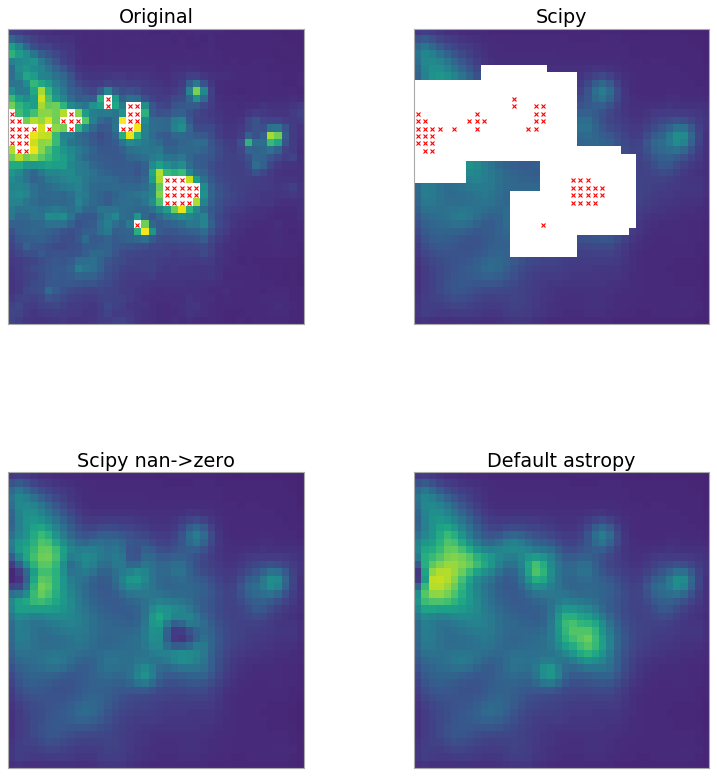
\includegraphics[width=\textwidth]{convolution_example.png}
\caption{%
    An example showing different modes of convolution available in the \python
    ecosystem.  The red x's mark pixels that are set to NaN in the original data
    (a).  If the data are convolved with a Gaussian kernel on a 9x9 grid using
    scipy's direct convolution (b), any pixel within range of the original NaN
    pixels is also set to NaN.  Panel (c) shows what happens if the NaNs are set
    to zero first: the originally NaN regions are depressed relative to their
    surroundings.  Finally, panel (d) shows \astropypkg's convolution behavior,
    where the missing pixels are replaced with values interpolated from their
    surroundings using the convolution kernel.
    \label{fig:convolution-example}
}
\end{figure}


\subsection{Visualization}
% Larry:  Image visualization (stretching, scaling), RGB

The \package{visualization} package provides functionality that can be helpful when visualizing data. This includes a framework for plotting astronomical images with coordinates with Matplotlib (previously the standalone \package{wcsaxes} package), functionality related to image normalization (including both scaling and stretching), smart histogram plotting, RGB color image creation from separate images, and custom plotting styles for Matplotlib.

\subsubsection{Image Stretching and Normalization}

\label{sec:stretch}

The \package{visualization} package provides a framework for transforming values in images (and more generally any arrays), typically for the purpose of visualization. Two main types of transformations are normalization and stretching of image values.

Normalization transforms the images values to the [0:1] range using lower and upper limits where $x$ represents the values in the original image:

\begin{equation}
y = \frac{x - v_{vmin}}{v_{max} - v_{min}}
\end{equation}

Stretching transforms the image values in the [0:1] range to the [0:1] range using a linear or non-linear function:
\begin{equation}
z = f(y)
\end{equation}

Several classes are provided for determining intervals (e.g. using image percentiles) and for normalizing values in this interval to the [0:1] range.

\package{Matplotlib} allows a custom normalization and stretch to be used when displaying data by passing a normalization object.  The \package{visualization} package also provides a normalization class that wraps the interval and stretching objects into a normalization object that \package{matplotlib} understands.

\subsubsection{Plotting image data with world coordinates}

One of the most common tasks by astronomers dealing with observational data is to make figures with images that include the correct coordinates and optionally with a coordinate grid. The challenge however is that the conceptual coordinate axes (such as longitude/latitude) need not be lined up with the pixel axes of the image. The \package{visualization.wcsaxes} subpackage implements a generalized way of making figures from an image array and a world coordinate system (WCS) object that provides the transformation between pixel and `world' coordinates. World coordinates can be for example right ascension and declination, but can also include for example velocity, wavelength, frequency, time, and so on. The main features from this subpackage include the ability to control which axes to show which coordinate on (for example showing longitude ticks on the top and bottom axes and latitude on the left and right axes), controlling the spacing of the ticks either by specifying the positions to use or providing a tick spacing or an average number of ticks that should be present on each axis, setting the format for the tick labels to ones commonly used by astronomers, controlling the visibility of the grid/graticule, and overlaying ticks, labels, and/or grid lines from different coordinate systems. In addition, it is possible to pass data with more than two dimensions and slice on-the-fly. Finally, it is possible to define non-rectangular frames, such as for example for Aitoff projections.

This subpackage differs from APLpy \citep{aplpy} in that the latter focuses on providing a very high-level interface to plotting that requires very few lines of code to get a good result, whereas WCSAxes defines an interface that is much closer to that of Matplotlib \citep{matplotlib}, and makes it possible to make significantly more advanced visualizations. An example of a visualization made with \package{wcsaxes} is shown in Figure~\ref{fig:wcsaxes} -- this example illustrates the ability to overlay multiple coordinate systems and customize which ticks/labels are shown on which axes around the image. This also uses the image stretching functionality from Section~\ref{sec:stretch} to show the image in a square root stretch (automatically updating the tick positions in the colorbar).

\begin{figure}
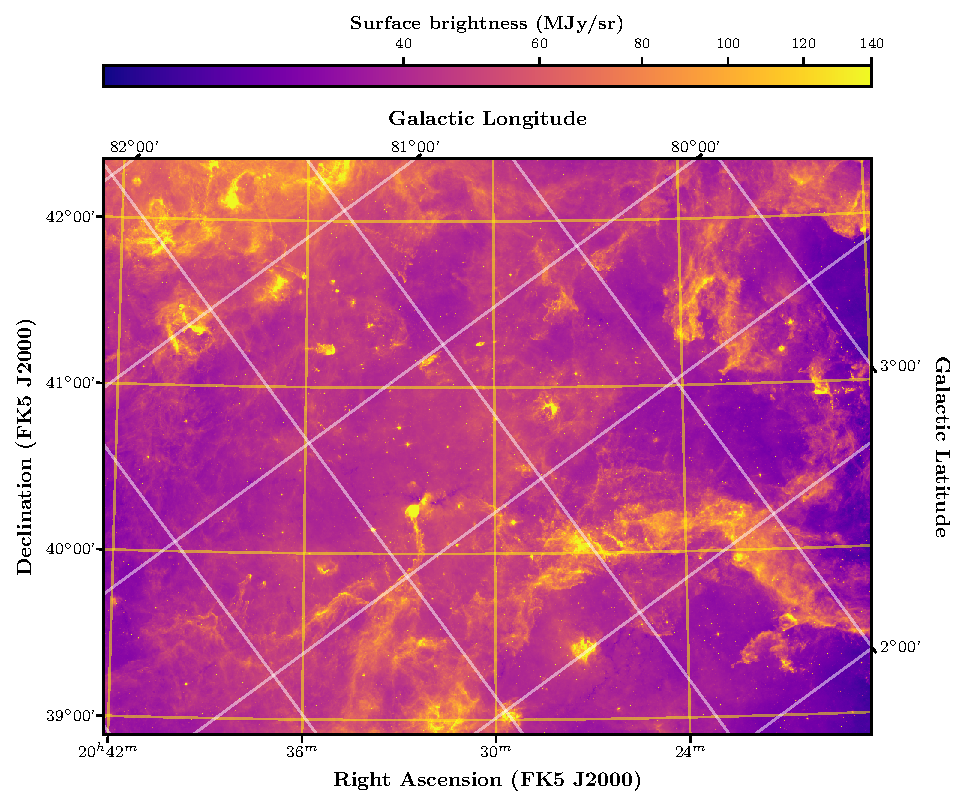
\includegraphics[width=\textwidth]{cygnus_x_spitzer.pdf}
\caption{%
An example of figure made using the \package{visualization.wcsaxes} subpackage, using \textit{Spitzer}/IRAC 8.0$\mu$m data from the Cygnus-X Spitzer Legacy survey \citep{cygnusx}.
\label{fig:wcsaxes}
}
\end{figure}

\subsubsection{Choosing Histogram Bins}

The package also provides the a histogram function, which is a generalization of \package{matplotlib}’s histogram function, to allow for more flexible specification of histogram bins.  The function provides several methods of automatically tuning the histogram bin size. It has a syntax identical \package{matplotlib}’s histogram function (with the exception of the bins parameter), which allows specification of one of four different methods for automatic bin selection.

\subsubsection{Creating color RGB images}

\cite{Lupton2004} describe an “optimal” algorithm for producing red-green-blue (RGB) composite images from three separate high-dynamic range arrays. The \package{visualization} package provides a convenience function to create such a color image.  It also includes an associated set of classes to provide alternate scalings.
This functionality was contributed by developers from the Large Synoptic Survey Telescope (LSST) and serves as an example of contribution to Astropy from a more traditional engineering organization \citep{lsst_astropy}.

The Sloan Digital Sky Survey (SDSS) SkyServer color images were made using a variation on this technique.  As an example, in \figurename~\ref{fig:ngc6977} we show an RGB color image of the Hickson 88 group, centered near NGC~6977.  This image was generated from SDSS images using the \package{astropy.visualization} tools.

\begin{figure}
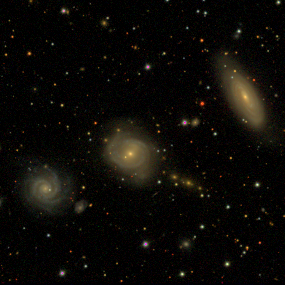
\includegraphics[width=\textwidth]{ngc6977.png}
\caption{An RGB color image of the region near the Hickson 88 group
constructed from SDSS images and the \package{astropy.visualization}
tools.
\label{fig:ngc6977}}
\end{figure}

%\subsection{Utils}
% Lim

\subsection{Cosmology}


\subsection{Statistics}

The \package{astropy.stats} package provides statistical tools that
are useful for or specific to astronomy and are not found in or extend
the available functionality of other \python\ statistics packages such
as \package{scipy} \citep{scipy} or \package{statsmodels}
\citep{seabold2010statsmodels}.  The \package{stats} package contains
a range of different functionality used by many different disciplines
in astronomy.  It is not a complete set of statistic tools, but rather
a still growing collection of useful features.

The current review process for contributions to the \package{stats} package includes review of the code, documentation, testing, and scientific merit of the inclusion.  When necessary, scientific reviewers outside of the maintainers will be sought for their input on new pull requests.

In this section, we describe these tools that provide a range of different functionality including robust statistical estimators, circular statistics, periodograms, spatial statistics, and histogram binning.


% Steve C.: overview, circular stats,
% Jake V.:  Lomb-scargle, Bayesian blocks
% Larry:  sigma clipping, biweight stats
% Ze':  Ripley's K (spatial stats)

\subsubsection{Robust Statistical Estimators}

Robust statistics provide reliable estimates of basic statistics for complex distributions that largely mitigate the effects of outliers. The \package{stats} package includes several robust statistical functions that are commonly used in astronomy. This includes sigma clipping methods for rejecting outliers, median absolute deviation functions, and biweight estimators, which have been used to calculate the velocity dispersion of galaxy clusters \citep{Beers1990}.

{\subsubsection{Circular Statistics}

A set of circular statistical estimators based on \citet{JammalamadakaSengupta}
are implemented in the \package{stats} package.  These functions provide
measurements of the circular mean, variance, and moment.   For all of these
functions, they work with both \texttt{numpy.ndarrays} (assumed to be in
radians) and \texttt{Quantity} objects.  In addition, the package includes
tests for Rayleigh Test \citep{wilkie83}, vtest [XXX], and a function to
compute the maximum likelihood estimator for the parameters of the von Mises
distribution [XXX].

\subsubsection{Lomb-Scargle Periodograms}
Periodic analysis of unevenly-spaced time series is common across subfields of Astronomy. The \package{stats} package now includes several efficient implementations of the Lomb-Scargle periodogram \citep{Lomb76, Scargle82} and several generalizations, including floating mean models \citep{Zechmeister09}, truncated Fourier models \citep{Bretthorst2003}, and appropriate handling of heteroscedastic uncertainties. Importantly, the implementations make use of several fast and scalable computational approaches \citep[e.g.][]{Press89, Palmer09}, and so can be applied to much larger datasets than Lomb-Scargle algorithms available in, e.g. \package{scipy.stats} (\citealt{scipy}). Much of the Lomb-Scargle code in AstroPy has been adapted from previously-published open-source code \citep{astroML, VanderPlas2015}.

\subsubsection{Bayesian Blocks and Histogram Binning}
AstroPy also includes an implementation of {\it Bayesian Blocks} \citep{Scargle2013}, an algorithm for analysis of break-points in non-periodic astronomical time-series. One interesting application of Bayesian Blocks is its use in determining optimal histogram binnings, and in particular binnings with unequal bin sizes. This code was adapted, with several improvements, from the \package{astroML} package \citep{astroML}. An example of a histogram fit using the Bayesian blocks algorithm is shown in the right panel of \figurename\ref{fig:bayes-blocks-hist}.

\begin{figure}
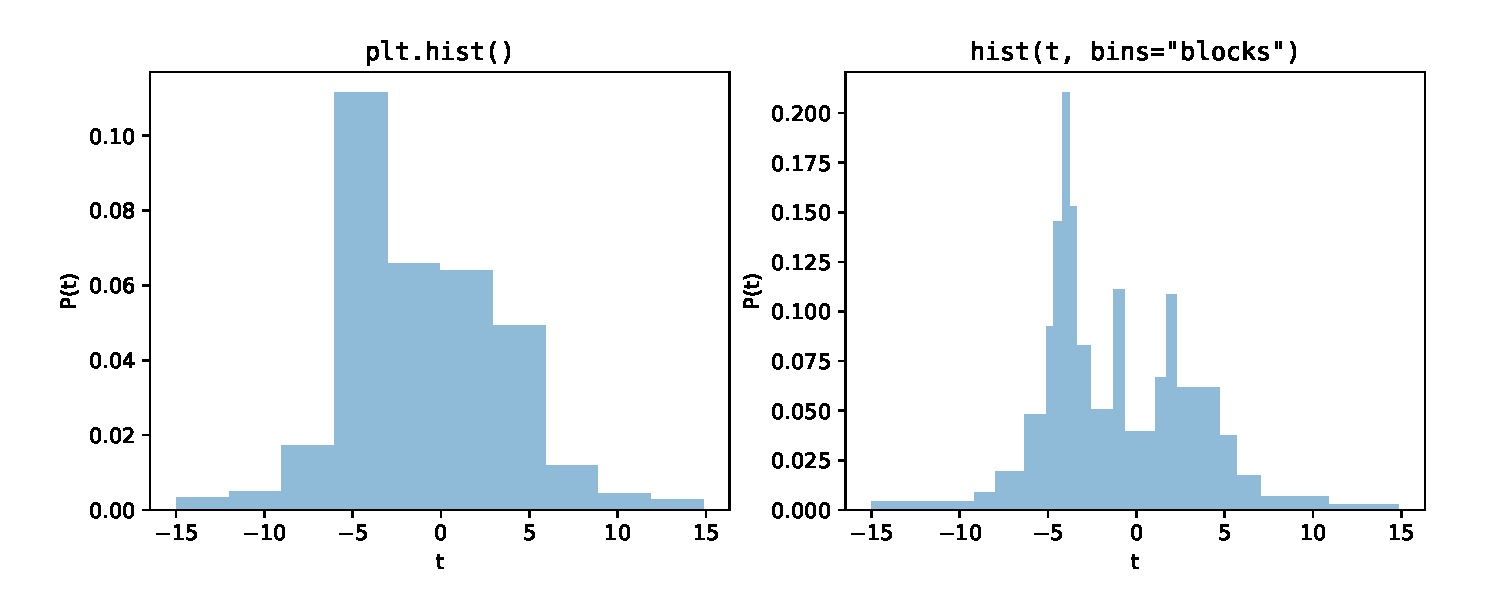
\includegraphics[width=\textwidth]{bayesian_blocks_hist.pdf}
\caption{%
    A histogram with irregular bins, fit using the Bayesian blocks
    algorithm. The left panel shows a standard histogram using
    \package{matplotlib}'s default of 10 bins. The right panel shows
    the same histogram with bin widths determined by the Bayesian
    blocks model. The model is such that relevant features of the data
    distribution are much more apparent.
    \label{fig:bayes-blocks-hist}
}
\end{figure}

\section{Infrastructure for affiliated packages}
\label{sec:infrastructure}
\inlinecomment{BMS}{should we use links to the appropriate github repo?}
\inlinecomment{PLL}{IMHO a list of GitHub repo links for affil. pkgs. should be in appendix, if included.}
\inlinecomment{BMS}{should we describe astropy-helpers even though it's future is unsure?}
%
\par In addition to astronomy related packages and libraries, the \astropy\
Project also contains and supports several infrastructure packages that are
very generic. The following sections describes the most widely used
selection of them.
%
\subsection{Package template}
% Brigitta may write this up if there is no other takers
\par \astropy provides a template package that any \python package is welcome to
use (many affiliated packages do so). The template contains a ready-to-go
package layout. It provides infrastructure such as documentation tools,
testing framework and CI templates and configurations, Cython integration,
and documentation on how to make it all work.
%
\subsection{Continuous integration helpers}
% Brigitta
\package{ci-helpers} is a collection of scripts that empowers package
maintainers to control their testing set up and installation process for
various continuous integration services via a set of environment
variables. While the current development is mostly driven by the needs of
the \astropy ecosystem, the actual usage of this package is extremely
widespread. Currently we support setups for Travis CI and Appveyor CI.
%
\subsection{Sphinx extensions}

The documentation for many Python packages the core \package{astropy} package as well as for all packages in the Astropy ecosystem is written using the Sphinx package. This package makes it possible to write the documentation using plain text files that follow a markup language called reStructuredText, and Sphinx can then transform this into HTML or \LaTeX documentation. As part of the project, we have developed a few extensions that facilitate generating documentation for a large project like Astropy. One of the main extensions we have developed is \package{sphinx-automodapi}\footnote{\url{http://sphinx-automodapi.readthedocs.io}}, which makes it easy with a single reStructuredText command to generate a set of documentation pages listing all the available classes, functions, and attributes in any given Python module.

\inlinecomment{TPR}{We should put the releases of sphinx-automodapi on Zenodo and cite this}

% TODO: need to put releases of sphinx-automodapi on Zenodo!

%\inlinecomment{BMS}{What about pytest-astropy, should we inlude it here, or
%  for the future section?}
%\inlinecomment{PLL}{pytest-astropy is v3, right?}
% \section{State of the Ecosystem}
% Commenting out unless a clear statement is added

%\section{Learning Astropy}
%\label{sec:learning}
% Kelle, Adrian
%\inlinecomment{BMS}{would astropy learn mature enough to described in the paper, or maybe it should go as a subsection for the next, future of astropy section?}

%Explain components: Documentation, Tutorials, and lessons

\section{The future of the Astropy project}
\label{sec:future}
\inlinecomment{PLL}{In addition to PY3, add some killer features that we
  plan to implement for 3.0 and beyond?}
\inlinecomment{BMS}{Some killer features we already know about to definitely
have may be mentioned here. e.g. functionality of astropy-healpix? or the
performance/speedup focus of the 3.1 release?}
\inlinecomment{BMS}{should we mention the refactored infra here?
  e.g. pytest-astropy and sphinx-astropy?}
\subsection{Roadmap for \python 3 only support}

dropping \python 2 support, growths of affiliated packages
Summary
learning astropy 

\section{Outlook}
\label{sec:outlook}
\inlinecomment{hamogu}{This may be merged into the section above once
  that is fleshed out a little more.}  As shown above the development
of the \astropypkg package is making good progress, helping
astronomers worldwide to perform many daily tasks such as planning
observations, analyzing data or simulation results, and writing
publications. The strong emphasis that the \astropy project puts on
reliability and code correctness helps users to trust the calculations
performed with \astropypkg and to publish reproducible results. More
functionality is added to the core package and more and more
affiliated packages support more specialized needs.

At the same time, \astropy is spreading awareness of best practices in
software development. This is important since most practicing
astronomers received their education without being taught in computer
science and software development although a major fraction of almost
every astronomer's workload today is related to software use and
development. The \astropypkg package leads by example, showing all interested
astronomers how modern tools like git version control or continuous
integration (code is tested after every change to the source) can
increase the quality and accessibility of astronomical software
without overly complicating the development cycle. All submitted code
is reviewed by at least one, but typically more, members of the
astropy community, providing feedback and allowing contributors to
improve their skill is developing software without the need for their
institutions to provide dedicated teaching resources. Thus, the
\astropy project does not only build the tools needed to perform
productive astronomical research in an era of increasingly large and
complex datasets, it also helps to prepare the current and the next
generation of researchers with the knowledge to adequately use those
tools.


\acknowledgments

Who to thank?  numfocus,

Software/services to thank: GitHub. Travis CI, Appveyor, CircleCI. Read the Docs.

%% Similar to \facility{}, there is the optional \software command to allow
%% authors a place to specify which programs were used during the creation of
%% the manusscript. Authors should list each code and include either a
%% citation or url to the code inside ()s when available.

\software{\package{astropy} (\citealt{astropy}),
          \package{numpy} (\citealt{numpy}),
          \package{scipy} (\citealt{scipy}),
          \package{matplotlib} (\citealt{matplotlib})
          \package{Cython}(\citealt{cython}),
          }

\bibliographystyle{aasjournal}
\bibliography{bibliography}


\appendix
\section{List of Affiliated Packages}

\begin{table}[h]
  \centering
  \caption{Registry of affiliated packages.}
  \label{tab:registry}
  \begin{tabular}{cccc}
    \toprule
    Package Name  & Stable & PyPI Name & Maintainer \\
    \midrule
      \href{https://github.com/astropy/astroscrappy}{Astro-SCRAPPY} & Yes & \href{https://pypi.python.org/pypi/astroscrappy}{astroscrappy} & Curtis McCully & \citealt{astroscrappy} \\
\href{https://github.com/astropy/astroplan}{astroplan} & No & \href{https://pypi.python.org/pypi/astroplan}{astroplan} & Brett Morris & \citealt{astroplan_AAS}\\
\href{http://github.com/astropy/astroquery}{astroquery} & Yes & \href{https://pypi.python.org/pypi/astroquery}{astroquery} & Adam Ginsburg and Brigitta Sipocz & \citealt{astroquery}\\
\href{http://github.com/astropy/ccdproc}{ccdproc} & Yes & \href{https://pypi.python.org/pypi/ccdproc}{ccdproc} & Steven Crawford, Matt Craig, and Michael Seifert & \citealt{ccdproc}\\
\href{https://github.com/jesford/cluster-lensing}{cluster-lensing} & No & \href{https://pypi.python.org/pypi/cluster-lensing}{cluster-lensing} & Jes Ford & \citealt{clusterlensing} \\
\href{https://github.com/adrn/gala}{gala} & Yes & \href{https://pypi.python.org/pypi/astro-gala}{astro-gala} & Adrian Price-Whelan & \citealt{gala}\\
\href{https://github.com/jobovy/galpy}{galpy} & Yes & \href{https://pypi.python.org/pypi/galpy}{galpy} & Jo Bovy & \citealt{galpy}\\
\href{http://github.com/gammapy/gammapy}{gammapy} & No & \href{https://pypi.python.org/pypi/gammapy}{gammapy} & Christoph Deil & \citealt{gammapy}\\
\href{http://github.com/ejeschke/ginga}{ginga} & Yes & \href{https://pypi.python.org/pypi/ginga}{ginga} & Eric Jeschke and Pey-Lian Lim & \citealt{ginga}\\
\href{https://github.com/glue-viz/glue}{Glue} & Yes & \href{https://pypi.python.org/pypi/glueviz}{glueviz} & Chris Beaumont and Thomas Robitaille & \citealt{glue}\\
\href{https://github.com/spacetelescope/gwcs}{gwcs} & No & \href{https://pypi.python.org/pypi/gwcs}{gwcs} & Nadia Dencheva & \citealt{gwcs}\\
\href{https://github.com/astropy/halotools}{Halotools} & Yes & \href{https://pypi.python.org/pypi/halotools}{halotools} & Andrew Hearin & \citealt{halotools}\\
\href{http://github.com/spacetelescope/imexam}{imexam} & No & \href{https://pypi.python.org/pypi/imexam}{imexam} & Megan Sosey & \\
\href{https://github.com/Chandra-MARX/marxs}{marxs} & Yes & \href{https://pypi.python.org/pypi/marxs}{marxs} & Hans Moritz Günther (hamogu) & \citealt{marxs}\\
\href{https://github.com/astropy/montage-wrapper}{montage-wrapper} & Yes & \href{https://pypi.python.org/pypi/montage-wrapper}{montage-wrapper} & Thomas Robitaille & \\
\href{https://github.com/zblz/naima}{naima} & Yes & \href{https://pypi.python.org/pypi/naima}{naima} & Victor Zabalza & \citealt{naima}\\
\href{http://github.com/astropy/photutils}{photutils} & No & \href{https://pypi.python.org/pypi/photutils}{photutils} & Larry Bradley and Brigitta Sipocz & \citealt{photutils} \\
\href{http://github.com/weaverba137/pydl}{PyDL} & No & \href{https://pypi.python.org/pypi/pydl}{pydl} & Benjamin Alan Weaver & \\
\href{https://github.com/olebole/python-cpl}{python-cpl} & No & \href{https://pypi.python.org/pypi/python-cpl}{python-cpl} & Ole Streicher & \\
\href{https://github.com/astrofrog/reproject}{reproject} & Yes & \href{https://pypi.python.org/pypi/reproject}{reproject} & Thomas Robitaille & \\
\href{http://github.com/sncosmo/sncosmo}{sncosmo} & Yes & \href{https://pypi.python.org/pypi/sncosmo}{sncosmo} & Kyle Barbary & \citealt{sncosmo}\\
\href{https://github.com/radio-astro-tools/spectral-cube}{spectral-cube} & Yes & \href{https://pypi.python.org/pypi/spectral-cube}{spectral-cube} & Adam Ginsburg & \citealt{spectralcube}\\
\href{http://github.com/astropy/specutils}{specutils} & No & \href{https://pypi.python.org/pypi/specutils}{specutils} & Nicholas Earl, Adam Ginsburg, Steve Crawford & \\

    \bottomrule
  \end{tabular}
\end{table}

\begin{table}[h]
  \centering
  \caption{Registry of provisionally accepted affiliated packages.}
  \label{tab:registry_prov}
  \begin{tabular}{cccc}
    \toprule
    Package Name  & Stable & PyPI Name & Maintainer \\
    \midrule
      \href{http://github.com/aplpy/aplpy.git}{APLpy} & Yes & \href{https://pypi.python.org/pypi/APLpy}{APLpy} & Thomas Robitaille and Eli Bressert \\
\href{http://github.com/astroML/astroML}{astroML} & Yes & \href{https://pypi.python.org/pypi/astroML}{astroML} & Jake Vanderplas \\
\href{https://github.com/StingraySoftware/HENDRICS}{HENDRICS} & Yes & \href{https://pypi.python.org/pypi/hendrics}{hendrics} & Matteo Bachetti \\
\href{https://github.com/RiceMunk/omnifit}{omnifit} & Yes & \href{https://pypi.python.org/pypi/omnifit}{omnifit} & Aleksi Suutarinen \\
\href{https://github.com/astropy/pyregion.git}{pyregion} & Yes & \href{https://pypi.python.org/pypi/pyregion}{pyregion} & Jae-Joon Lee \\
\href{https://github.com/pyvirtobs/pyvo.git}{PyVO} & No & \href{https://pypi.python.org/pypi/pyvo}{pyvo} & Stefan Becker \\
\href{https://github.com/spacetelescope/spherical_geometry.git}{spherical\_geometry} & No & \href{https://pypi.python.org/pypi/spherical-geometry}{spherical-geometry} & Bernie Simon and Michael Droettboom \\

    \bottomrule
  \end{tabular}
\end{table}

\end{document}

